\subsection{DC Inversion of the forward model}
We use several synthetic examples to illustrate various aspects of \prog. The emphasis of the test examples is to show the newly added features of the inversion programs. A synthetic conductivity model is shown in Figure \ref{fig:fwdAR} and resultant synthetic data I shown in Figure \ref{fig:fwdTrueCrop}.

The synthetic model consists of two conductors buried in a uniform half space, which is overlain by an overburden of variable conductivity. A V-shaped valley is cut out to simulate the surface topography. The background has a conductivity of 1 mS/m and the overburden has a conductivity of 0.1 mS/m on the left and 2 mS/m on the right. The buried conductor on the left has a dip of 135o and a conductivity of 100 mS/m, and it is buried at a depth of 20 m to the top. The conductor on the right is a horizontal and conductive block of 100 mS/m buried at a depth of 25 m. The forward modelling uses a mesh of 48 cells in the x-direction and 27 cells in the z-direction so there are 1296 cells. In the survey, surface electrodes are located every 10 m in the interval $x=(-100,100)$ m. We have simulated pole-dipole data with a=10 m and n=1, 8. The data have been contaminated with independent Gaussian noise whose standard deviation is equal to 5\% of each accurate datum.

We have carried out nine DC inversions of the above DC data set. The examples were designed to illustrate the performance of the inversion program when different combinations of input parameters are used.

\subsubsection{DC Inversion: All default}
First, the synthetic data were inverted using the all-default option:
%
\begin{fileExample}
\begin{tabular}{|ll|}
\hline
OBS LOC\_X obs\_dc.dat & ! DC data \\
TOPO FILE topo.dat & ! Topography\\
MESH FILE dcinv2d.msh & ! Mesh\\
\hline
\end{tabular}
\end{fileExample}
%
In this file, the first line indicates that the data file \fileName{obs\_dc.dat} is of \fileName{surface} format. The second line contains the reference to topography file \fileName{topo.dat}. The third line is in reference to the mesh file ]\fileName{dcinv2d.msh}. If there is no topography it is not necessary to include either the mesh, or the topography file in all-default mode. \prog~will construct a mesh in automatic mode and consider topography to be zero. In our case we have user-defined topography and mesh file is provided. The result of the all-default inversion is shown in Figure \ref{fig:alldefault}. The best fitting half space was approximately 120 ohm-m.
%
\begin{figure}
\centering
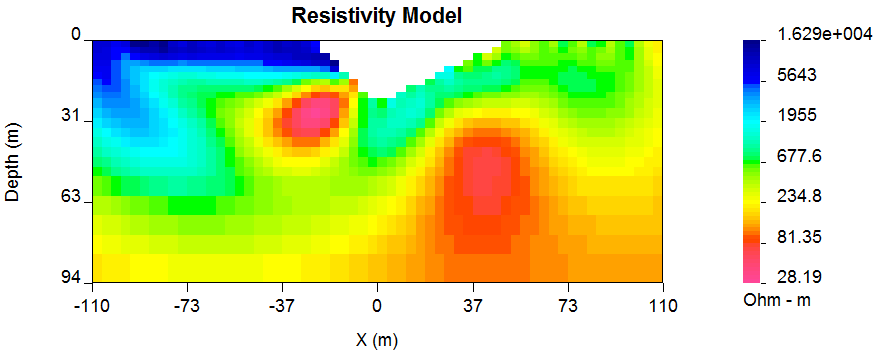
\includegraphics[width=0.5\columnwidth]{alldefault}
\caption{Inversion of synthetic DC data using all-default mode.}
\label{fig:alldefault}
\end{figure}

\subsubsection{DC Inversion: CG solution using a constant reference model}
In the next example, definition of some parameters has been set to user-defined and changed. In real life this can be done if there is a higher level of certainty regarding some starting parameters (prior information). The control file for the next example is provided below:
%
\begin{fileExample}
\begin{tabular}{|ll|}
\hline
OBS LOC\_X obs\_dc.dat & ! DC data \\
TOPO FILE topo.dat & ! Topography\\
MESH FILE dcinv2d.msh & ! Mesh \\
ALPHA VALUE 1.e-3 1.0 1.0 & ! Alphas \\
INVMODE CG & ! Use CG \\
REF\_MOD VALUE 1.e-3 & ! Reference model \\
INIT\_MOD VALUE 1.e-3 & ! Initial model \\
\hline
\end{tabular}
\end{fileExample}
%
In this example, the fourth line indicates that the smallness coefficient ($\alpha_s$) is now user-defined (set to 0.001). The fifth line means that the system solver has been switched from default (Singular Value Decomposition or SVD solver) to the Conjugate Gradient solver (CG). The reference model has been set to 0.001 S/m (or 1000 Ohm m). The initial model has been set to the same as reference model. The results of applying these control file parameters are shown in the inversion model in Figure \ref{fig:synEx2}.
%
\begin{figure}
\centering
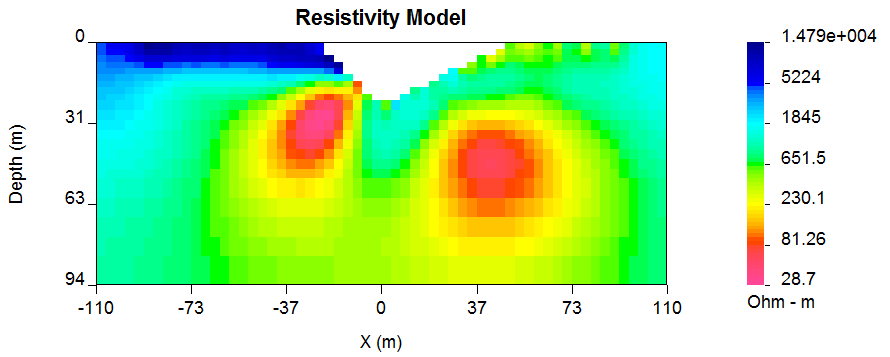
\includegraphics[width=0.5\columnwidth]{synEx2}
\caption{Inversion of synthetic DC data using user-defined smallness parameter ($\alpha_s$s) 1000 Ohm m half space as both: reference and a starting model.}
\label{fig:synEx2}
\end{figure}

The basic features of the models in Figure \ref{fig:alldefault} and Figure \ref{fig:synEx2} are similar. Both conductors have been located and so has the resistive overburden on the left. (Compare with the synthetic model in Figure \ref{fig:fwdTrueCrop}). Nevertheless, there are differences. Figure \ref{fig:synEx2}, which uses a more resistive reference model, supports the interpretation of closure for the body on the right. There is also an odd structure emanating from the left most part of the resistive overburden observed in Figure \ref{fig:alldefault} that is not observed in Figure \ref{fig:synEx2}. The primary differences between the two models can be explained through the use of a DOI (Depth of Investigation) plot. For the present we use Figure \ref{fig:synEx2} as a reference and Figure \ref{fig:alldefault} as an additional model. 

When the inversion volume is cut with respect to the DOI, then differences in the images are no longer so apparent. For the remainder of the example section we shall use the reference the model described in Figure \ref{fig:synEx2} (1000 Ohm m half space) as the \fileName{default} model.

\subsubsection*{Depth of Investigation (DOI)}
Models produced by inversion of DC resistivity data tend to approach the background conductivity of the reference model. At those depths the recovered model is no longer being influenced by the data. We can use this result to help estimate our depth of investigation. If there are at two reasonable models obtained using different reference models, the two models can be compared to identify which regions of the model are most significantly affected by the measurements. The results of doing this are explained next.

Using \prog, the method is applied within the \codeName{DCIP2D-MODEL-VIEWER} GUI, using \fileName{Depth of investigation} option in the \fileName{Options} menu. There must be a second model that was recovered using the same mesh as the one being observed. Any two different inversions results can be used. Here we use 1000 Ohm-m halfspace as our \fileName{best} model and we want blank out those sections of the model that are not well controlled by the data. A second inversion using a background of 106 Ohm-m (the default value from the code) and used that to compute the DOI. In Figure \ref{fig:doiInv}(a-b) shows the model with cutoffs of 0.1 and 0.4.
%
\begin{figure}
\centering
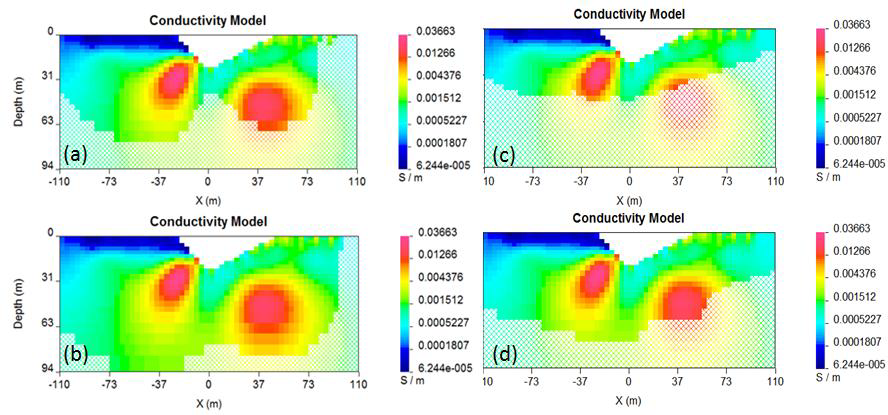
\includegraphics[width=0.5\columnwidth]{doiInvExample}
\caption{Assessing the depth of investigation (DOI): (a) based on recovered model (cut-off=0.1), (b) based on recovered model (cut-off = 0.4), (c) based on sensitivity (cut-off = 0.5), and (d) based on sensitivity (cut-off = 0.6).}
\label{fig:doiInv}
\end{figure}

Another option to assess the depth of investigation is through the analysis of the sensitivities. In \prog~there is a capability to visualize the sensitivities using the \codeName{DCIP2D-MODEL-VIEWER} GUI (Figure \ref{fig:doiInv}c and Figure \ref{fig:doiInv}d). Generally, the lower sensitivities correspond to less reliable model parameters (deeper-seated cells); higher sensitivities correspond to those model cells, which have most effect on the data (usually closer to surface). A good way to assess the DOI is by plotting the model on the full mesh extent (including the padding cells, Figure 19). In this figure we use the DOI evaluated from 1000 and 106 Ohm-m half spaces (that is, the same as Figure \ref{fig:doiInv}a and Figure \ref{fig:doiInv}b). As the DOI threshold decreases we limit the region of the model to that which is most controlled by the data. See (Figure \ref{fig:doiInvSens}a-c). The final choice of cutoff is selected by the user.
%
\begin{figure}
\centering
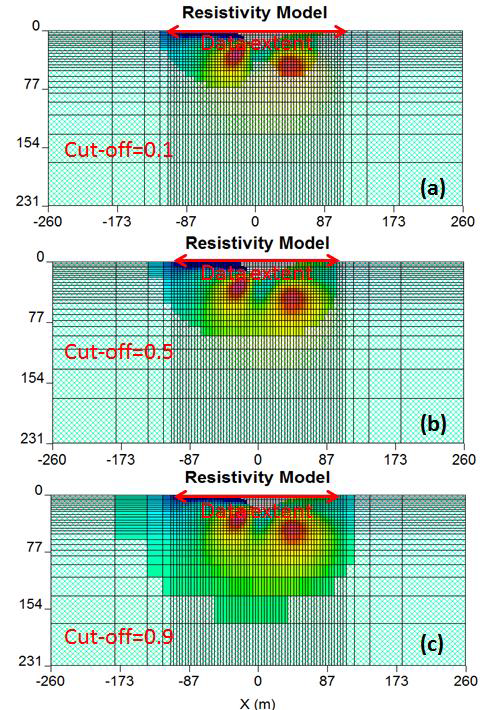
\includegraphics[width=0.5\columnwidth]{doiSensInvExample}
\caption{Assessing the depth of investigation (DOI): (a) based on recovered model (cut-off=0.1), (b) based on recovered model (cut-off = 0.4), (c) based on sensitivity (cut-off = 0.5), and (d) based on sensitivity (cut-off = 0.6).}
\label{fig:doiInvSens}
\end{figure}

\subsubsection{DC Inversion: Non-uniform reference model}
The next example is very similar to the previous inversion, with an exception that a different reference model is introduced (Figure \ref{fig:exRef}). As opposed to the previous example, where the reference model was set to a 1000 Ohm m half space, the new model includes an elongated conductive (10 Ohm m) rectangular block. The elongated block has the same value as the conductivity anomaly but the boundaries do not coincide. Moreover the block in the true model has smoothed boundaries. In summary, the supplied reference model has captured some aspects of the true conductivity but it is not an exact reflection of what is there. This example has been contrived to illustrate what happens with the options of including, or omitting, the reference model in derivative terms in the objective function according to equations \ref{eq:disMOF} and \ref{eq:mofNOref}.
%
\begin{figure}
\centering
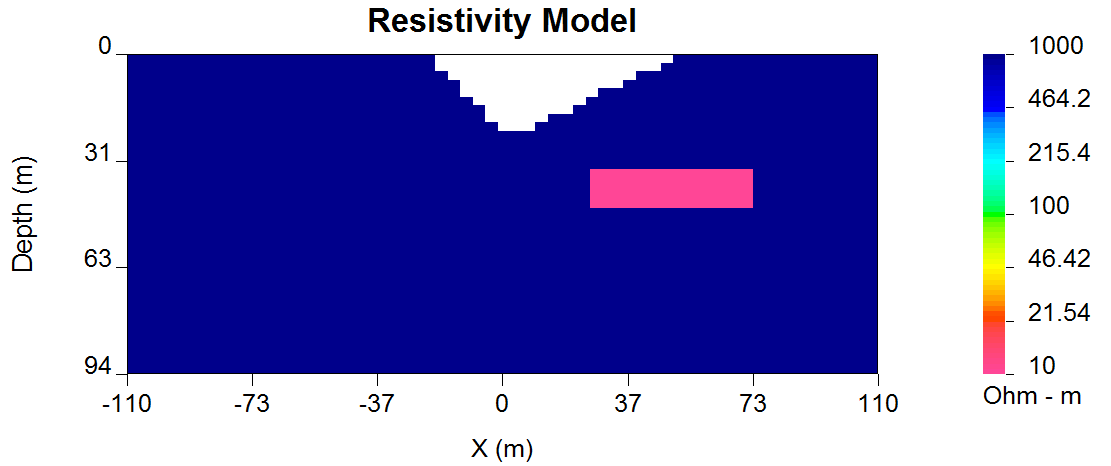
\includegraphics[width=0.5\columnwidth]{synRef}
\caption{Reference model applied for the synthetic example illustration.}
\label{fig:exRef}
\end{figure}

In the first example (control file provided below) the reference model was used in only the smallest model component.
%
\begin{fileExample}
\begin{tabular}{|ll|}
\hline
OBS LOC\_X obs\_dc.dat & ! DC data \\
TOPO FILE topo.dat & ! Topography\\
MESH FILE dcinv2d.msh & ! Mesh \\
ALPHA VALUE 1.e-2 1.0 1.0 & ! Alphas \\
INVMODE CG & ! Use CG \\
USE\_MREF FALSE & ! Ref out of spatial terms \\
REF\_MOD FILE new\_ref.con & ! Reference model \\
INIT\_MOD VALUE 1.e-3 & ! Initial model \\
NITER 40 & ! Max iterations \\
\hline
\end{tabular}
\end{fileExample}
%
In this control file line 7 now indicates that the reference model should be read from a file, rather than assigned a constant value; line 6 indicates that the reference model should be defined in non-derivative terms and line 9 is indicating that the maximum number of iterations for this inversion should not exceed 40. The results of this inversion can be seen in Figure /ref{fig:synWithRef}.
%
\begin{figure}
\centering
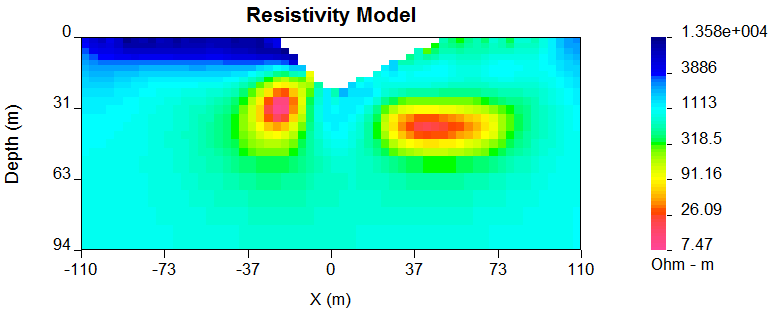
\includegraphics[width=0.5\columnwidth]{synWithRef}
\caption{Reference model applied for the synthetic example illustration.}
\label{fig:synWithRef}
\end{figure}

This is a superior model compared to that in Figure \ref{fig:synEx2}. The magnitude of the conductive anomaly is much better recovered, although at 7.6 Ohm-m it is slightly less resistive than the true value of 10 Ohm-m. It has a well-defined elongated shape with steep gradational boundaries that are good representations of the true model.
If we are more confident in the locations of the boundaries of the block in the reference model, then this can be incorporated into the inversion. We next carry out an inversion in which the reference model is included in the derivative terms. Below is the control file used for this inversion.
%
\begin{fileExample}
\begin{tabular}{|ll|}
\hline
OBS LOC\_X obs\_dc.dat & ! DC data \\
TOPO FILE topo.dat & ! Topography\\
MESH FILE dcinv2d.msh & ! Mesh \\
ALPHA VALUE 1.e-2 1.0 1.0 & ! Alphas \\
INVMODE CG & ! Use CG \\
REF\_MOD FILE new\_ref.con & ! Reference model \\
INIT\_MOD VALUE 1.e-3 & ! Initial model \\
NITER 40 & ! Max iterations \\
\hline
\end{tabular}
\end{fileExample}
%
The line (\codeName{USE\_MREF\_FALSE}) from the previous example has been eliminated, switching the inversion into the default mode (reference model is defined in the derivative terms in default mode). This line also could have been changed to \codeName{USE\_MREF\_TRUE}).

The result is shown in Figure \ref{fig:synWithRefIn} and it produces a model that has boundaries at the same location as the reference block and there is even more over-shoot of the conductivity. For this example however, putting in the reference model into the derivative terms is stronger information than is justified. In most cases, the previous solution, where the reference model was left out of the derivative terms is preferable.
%
\begin{figure}
\centering
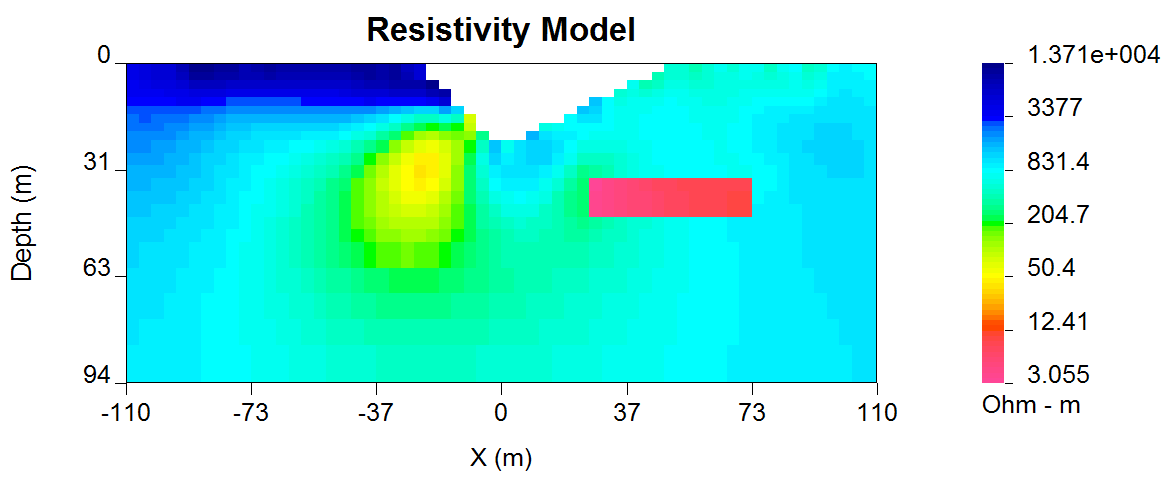
\includegraphics[width=0.5\columnwidth]{synWithRefIn}
\caption{Reference model applied for the synthetic example illustration.}
\label{fig:synWithRefIn}
\end{figure}

This is not always the case. Consider a situation where the goal is to find a body beneath an overburden layer. The model and the reference model are shown in Figure \ref{fig:synOverBurdenTrue}. It might be supposed that information about the overburden thickness and its resistivity have been obtained through drilling. Two inversions are carried out. In the first (Figure \ref{fig:synOverBurden}a) the reference model is omitted from the derivative term and the overburden boundary is characterized by a smooth transition. In the second case (Figure \ref{fig:synOverBurden}b) the reference model is included in the derivative terms and the result is a cleaner delineation of the overburden and better definition of the sought body.
%
\begin{figure}
\centering
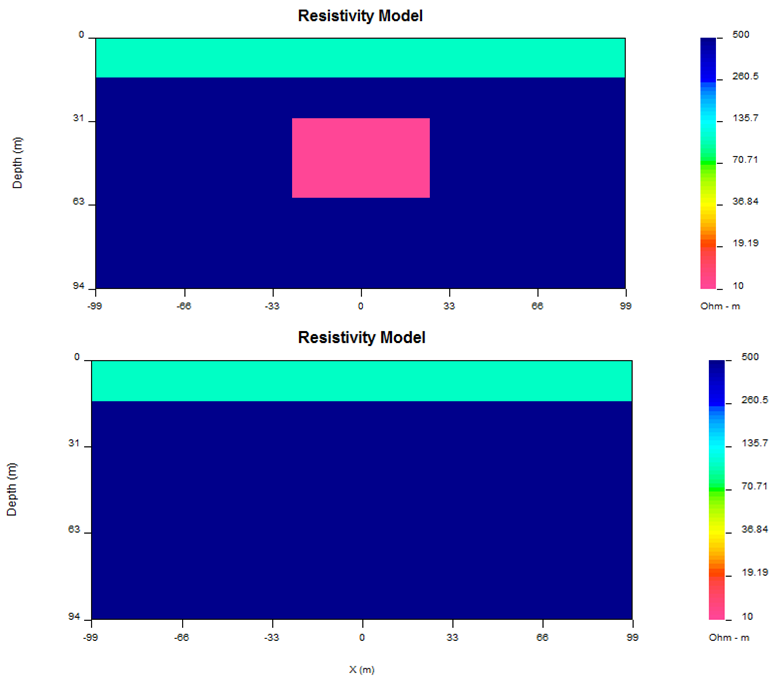
\includegraphics[width=0.5\columnwidth]{synOverBurdenTrue}
\caption{A conductive block underneath the overburden: (a) the true model and (b) the reference model.}
\label{fig:synOverBurdenTrue}
\end{figure}

\begin{figure}
\centering
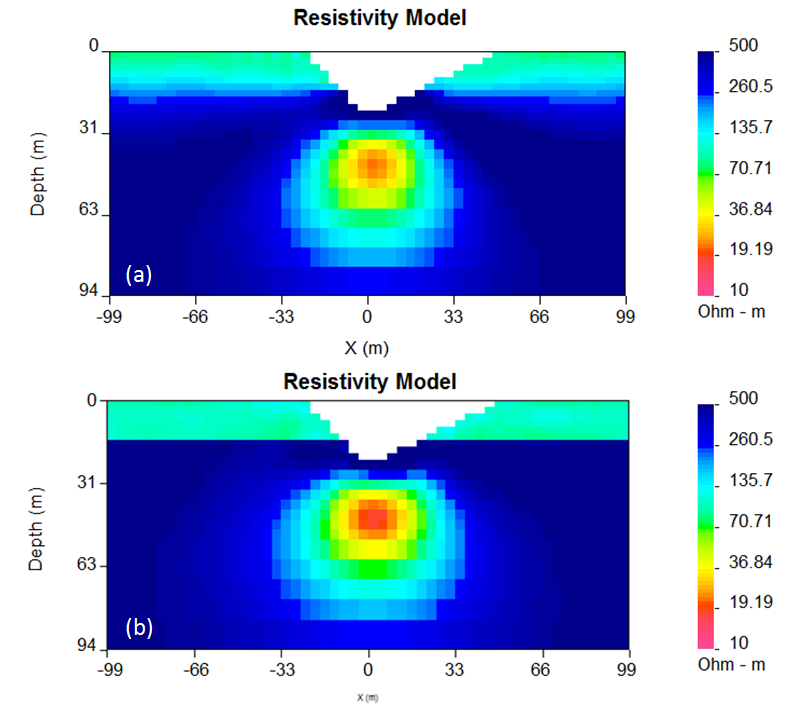
\includegraphics[width=0.5\columnwidth]{synOverBurden}
\caption{Inversion results when (a) the reference model is not included in the derivative terms and when (b) the reference model is defined in derivative terms.}
\label{fig:synOverBurden}
\end{figure}

\subsubsection{DC Inversion: Incorporating inactive cells constraint}
In the next example it is illustrated how drilling data can be incorporated in the inversion using fixed cells constraint. In this example, the reference model has been set to the same elongated conductive block model as shown in Figure \ref{fig:synOverBurdenTrue}. The difference is that in this case additional information has been incorporated by fixing some reference model cell values. The values are taken from the reference model file (\fileName{ref\_new.con}) but their values are fixed using active cells file (\codeName{ACTIVE\_CELLS active.txt}), defined in line 6 of the control file provided below.
%
\begin{fileExample}
\begin{tabular}{|ll|}
\hline
OBS LOC\_X obs\_dc.dat & ! DC data \\
TOPO FILE topo.dat & ! Topography\\
MESH FILE dcinv2d.msh & ! Mesh \\
ALPHA VALUE 1.e-3 1.0 1.0 & ! Alphas \\
INVMODE CG & ! Use CG \\
REF\_MOD FILE new\_ref.con & ! Reference model \\
INIT\_MOD VALUE 1.e-3 & ! Initial model \\
ACTIVE\_CELLS active.txt & ! Active cells \\
\hline
\end{tabular}
\end{fileExample}
%
The \fileName{active} file format was previously discussed within the \fileName{model} subsection in the \fileName{Elements} section of the manual, however another example is provided below:
%
\begin{fileExample}
\begin{tabular}{|cccccccccccccc|}
\hline
1 & 1 & 1 & 1 & 1 & 1 & 1 & 1 & 1 & 1 & 1 & 1 & 1 & 1 \\
1 & 1 & 1 & 1 & 1 & 1 & 1 & 1 & 1 & 1 & 1 & 1 & 1 & 1 \\
1 & 1 & 1 & 1 & 0 & 0 & 0 & 0 & 1 & 1 & 1 & 1 & 1 & 1 \\
1 & 1 & 1 & 1 & 0 & 0 & 0 & 0 & 1 & 1 & 1 & 1 & 1 & 1 \\
1 & 1 & 1 & 1 & 0 & 0 & 0 & 0 & 1 & 1 & 1 & 1 & 1 & 1 \\
1 & 1 & 1 & 1 & 1 & 1 & 1 & 1 & 1 & 1 & 1 & 1 & 1 & 1 \\
1 & 1 & 1 & 1 & 1 & 1 & 1 & 1 & 1 & 1 & 1 & 1 & 1 & 1 \\
\hline
\end{tabular}
\end{fileExample}
%
The format of this file is consistent with the model file, and the values equal to 1 define the model cells marked as \fileName{active}, while values equal to 0 define the model cells marked as \fileName{inactive} (without the capability affect the neighbouring cells). The case when inactive cells do not influence their neighbours is shown in Figure \ref{fig:synAct}.
%
\begin{figure}
\centering
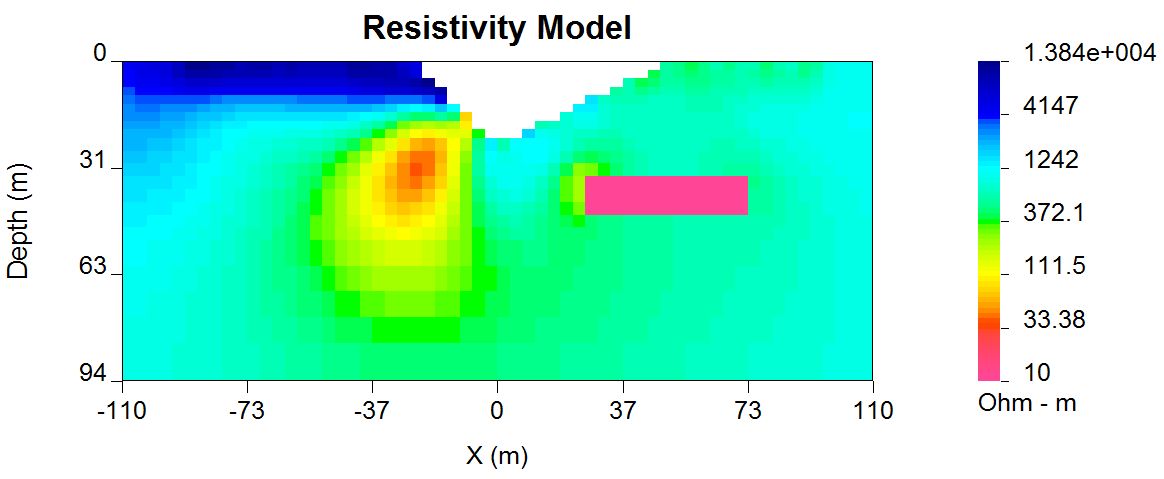
\includegraphics[width=0.5\columnwidth]{synAct}
\caption{Recovered model when the reference model cells are inactive and they do not influence the neighbouring cells.}
\label{fig:synAct}
\end{figure}

If it is desired to have the inactive cells influence the values of neighboring cells, then their values are set to -1 as in the file below. The resultant inversion model is shown in Figure \ref{fig:synAct2}. The region of high conductivity has been extended away from the reference model and the anomaly smoothly transitions to the background.
%
\begin{fileExample}
\begin{tabular}{|cccccccccccccc|}
\hline
1 & 1 & 1 & 1 & 1 & 1 & 1 & 1 & 1 & 1 & 1 & 1 & 1 & 1 \\
1 & 1 & 1 & 1 & 1 & 1 & 1 & 1 & 1 & 1 & 1 & 1 & 1 & 1 \\
1 & 1 & 1 & 1 & -1 & -1 & -1 & -1 & 1 & 1 & 1 & 1 & 1 & 1 \\
1 & 1 & 1 & 1 & -1 & -1 & -1 & -1 & 1 & 1 & 1 & 1 & 1 & 1 \\
1 & 1 & 1 & 1 & -1 & -1 & -1 & -1 & 1 & 1 & 1 & 1 & 1 & 1 \\
1 & 1 & 1 & 1 & 1 & 1 & 1 & 1 & 1 & 1 & 1 & 1 & 1 & 1 \\
1 & 1 & 1 & 1 & 1 & 1 & 1 & 1 & 1 & 1 & 1 & 1 & 1 & 1 \\
\hline
\end{tabular}
\end{fileExample}
%
\begin{figure}
\centering
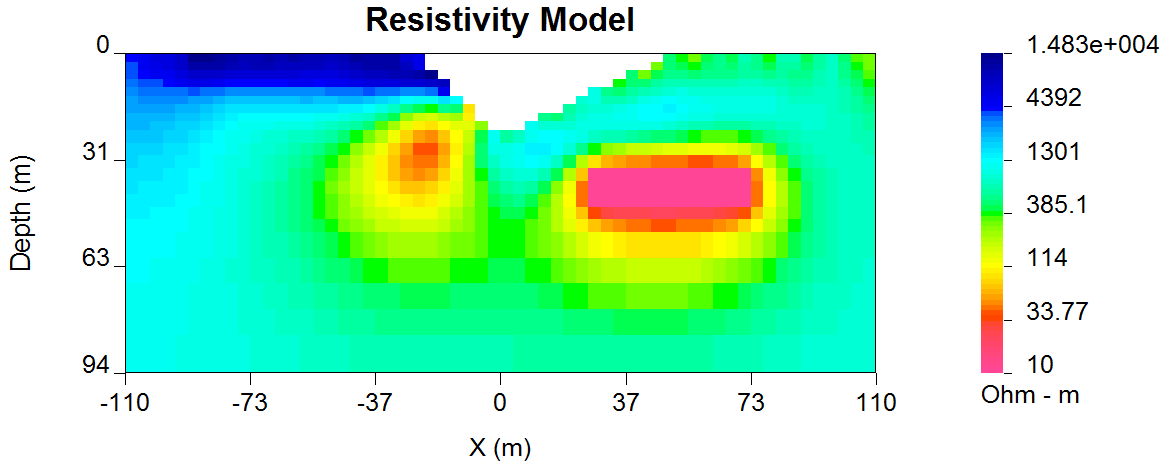
\includegraphics[width=0.5\columnwidth]{synAct2}
\caption{Recovered model when cells are inactive, but their values influence those of the neighbouring cells.}
\label{fig:synAct2}
\end{figure}

\subsubsection{DC inversion: Using weighting functions}
The next example illustrates the situation when prior information is incorporated using the \fileName{weighting} function file. The synthetic model for this example is the same as illustrated in Figure \ref{fig:synOverBurdenTrue}. Instead of reference model, a \fileName{weighting} file was used. The control file used for this inversion is shown below. The reference to the weighting file is provided in line 11 (\codeName{WEIGHT W.DAT}).
%
\begin{fileExample}
\begin{tabular}{|ll|}
\hline
OBS LOC\_X obs\_dc.dat & ! DC data \\
TOPO FILE topo.dat & ! Topography\\
MESH FILE dcinv2d.msh & ! Mesh \\
ALPHA VALUE 1.e-3 1.0 1.0 & ! Alphas \\
INVMODE CG & ! Use CG \\
REF\_MOD FILE 2e-3 & ! Reference model \\
INIT\_MOD VALUE 2e-3 & ! Initial model \\
USE\_MREF FALSE & ! Ref out of spatial terms  \\
WEIGHT w.dat & ! Weighting file \\
CHIFACT 1 & ! Chi factor of 1 \\
NITER 50 & ! Max iterations \\
\hline
\end{tabular}
\end{fileExample}

The recovered model is illustrated in Figure \ref{fig:synOverBurdenWght} and is very similar to the model shown in Figure \ref{fig:synOverBurden}b. The alternative of using a weighting file instead of the reference model facilitated the technical implementation of the prior constraints and brings an additional degree of freedom in being able to adjust the level of certainty in the a priori information by editing the weighting coefficients. In our case, the weighting coefficients were edited for the $\bvec{W}_z$ matrix, where the sixth interface (corresponding to the bottom of the overburden) was set to 0.1 (as opposed to default weights of 1.0).	
%
\begin{figure}
\centering
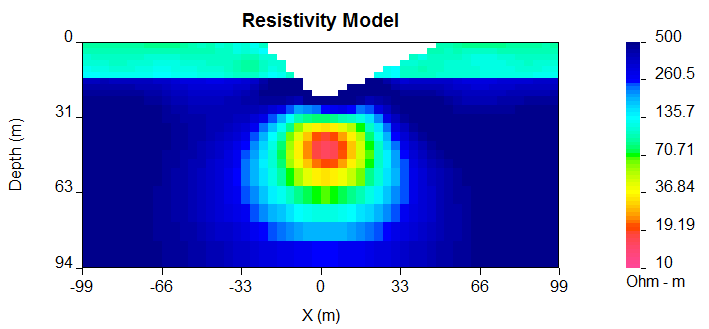
\includegraphics[width=0.5\columnwidth]{synOverBurdenWght}
\caption{Recovered model from the inversion using \fileName{weighting} file}
\label{fig:synOverBurdenWght}
\end{figure}

\subsubsection{DC Inversion: Using the Huber norm for data misfit}
The next example illustrates the effects that large data errors can have on the inversion and how these can be ameliorated with the Huber norm. The data are the same as used in previous examples except that 5 data have been severely perturbed. The inversions are carried out with the same standard deviation estimates, as used previously, a 1000 ohm-m background, and a data file contaminated with bad apparent resistivity values. Figure \ref{fig:huberCont} shows the contamination introduced to the apparent resistivity file used for the inversions.
%
\begin{figure}
\centering
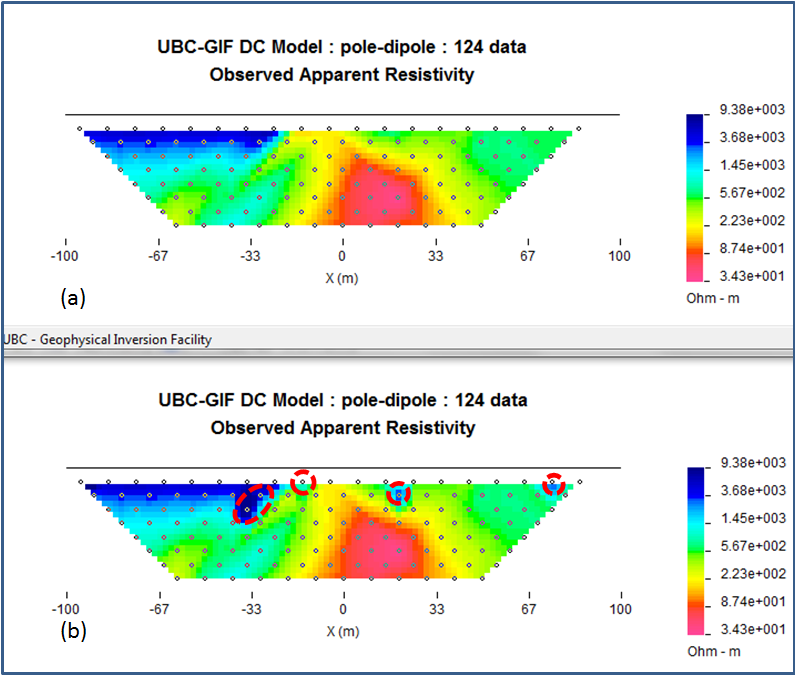
\includegraphics[width=0.5\columnwidth]{huberCont}
\caption{The (a) true data and (b) data contaminated with noise that will be inverted.}
\label{fig:huberCont}
\end{figure}

The contaminated data were inverted using a standard $l_2$ norm for the data misfit. The control file for this inversion is provided below:
%
\begin{fileExample}
\begin{tabular}{|ll|}
\hline
OBS LOC\_X obs\_dc.dat & ! DC data \\
TOPO FILE topo.dat & ! Topography\\
MESH FILE dcinv2d.msh & ! Mesh \\
ALPHA VALUE 1.e-3 1.0 1.0 & ! Alphas \\
INVMODE CG & ! Use CG \\
REF\_MOD FILE 1e-3 & ! Reference model \\
INIT\_MOD VALUE 1e-3 & ! Initial model \\
USE\_MREF TRUE & ! Ref everywhere  \\
WEIGHT w.dat & ! Weighting file \\
CG\_PARAM 20 1.e-2 & ! CG max iter and tol \\
NITER 20 & ! Max iterations \\
\hline
\end{tabular}
\end{fileExample}
%
The results of the inversion are shown in Figure \ref{fig:synHuberInv}. The inversion ran for 20 iterations and the target misfit was not achieved and there were many artifacts. The reason is that the great effort was being made to fit the five erroneous data.
%
\begin{figure}
\centering
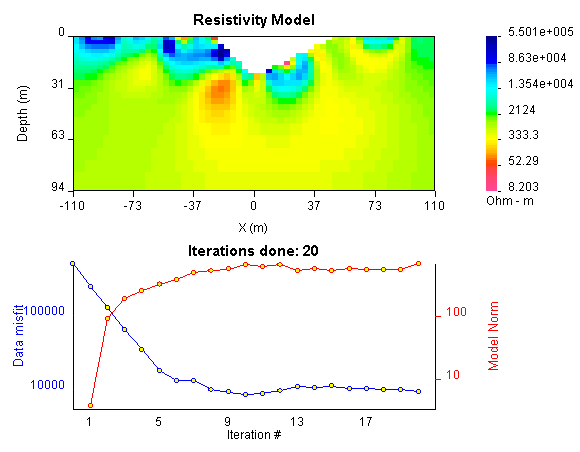
\includegraphics[width=0.5\columnwidth]{synHuberInv}
\caption{Recovered model (top) and conversion curves (bottom) from the inversion of the contaminated data. The data misfit utilized an $l_2$ norm.}
\label{fig:synHuberInv}
\end{figure}

In Figure \ref{fig:synHuberData} we show the observed data and the normalized misfit. Three of the five outliers are distinct and they contribute a value of 2067.05 to the final misfit of 9303. By recognizing them as outliers, they might be winnowed from further analysis but two erroneous data have been over fit by the modeling and as a result produced incorrect structure. This has led to other, higher quality data, having large misfits. This is characteristic of non-robust norms.
%
\begin{figure}
\centering
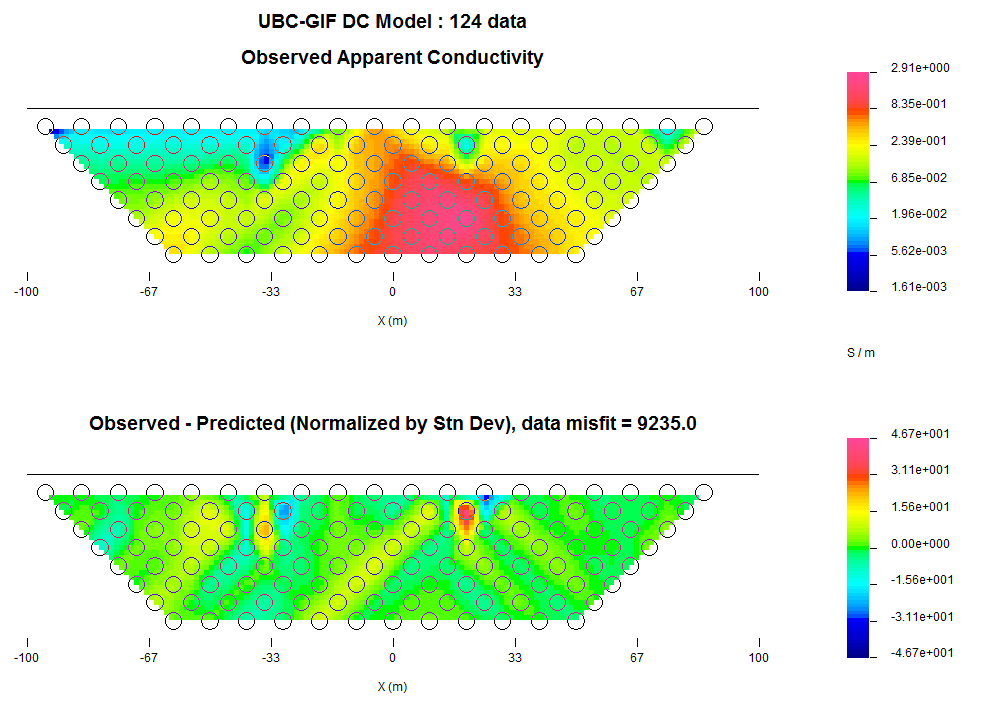
\includegraphics[width=0.5\columnwidth]{synHuberData}
\caption{Observed data (top) and the normalized difference (bottom) from the inversion using an $l_2$ misfit measure.}
\label{fig:synHuberData}
\end{figure}

In order to combat the effect that outliers in the data file may have on fitting the data using the $l_2$ measure, Huber norm was imposed on the data fit. The example of the control file with Huber norm is shown below:
%
\begin{fileExample}
\begin{tabular}{|ll|}
\hline
OBS LOC\_X obs\_dc.dat & ! DC data \\
TOPO FILE topo.dat & ! Topography\\
MESH FILE dcinv2d.msh & ! Mesh \\
ALPHA VALUE 1.e-3 1.0 1.0 & ! Alphas \\
INVMODE CG & ! Use CG \\
REF\_MOD FILE 1e-3 & ! Reference model \\
INIT\_MOD VALUE 1e-3 & ! Initial model \\
USE\_MREF FALSE & ! Ref out of spatial terms \\
HUBER 0.1 & ! Huber constant \\
NITER 40 & ! Max iterations \\
\hline
\end{tabular}
\end{fileExample}
%
Line 9 in this control file has been set to so that all normalized data misfits with value greater than 0.1 will be evaluated with the $l_1$ measure. The results are shown in Figure \ref{fig:synInvHuber2} and they appear much better, than in previous case. Nevertheless, they can still be improved by recognizing the existence of the highly erroneous data and winnowing them from the inversion.
incorrect structure. This has led to other, higher quality data, having large misfits. This is characteristic of non-robust norms. Although the recovery is far from perfect, the main conductor bodies are now shown with satisfactory detail, comparing to the $l_2$ normalization.
%
\begin{figure}
\centering
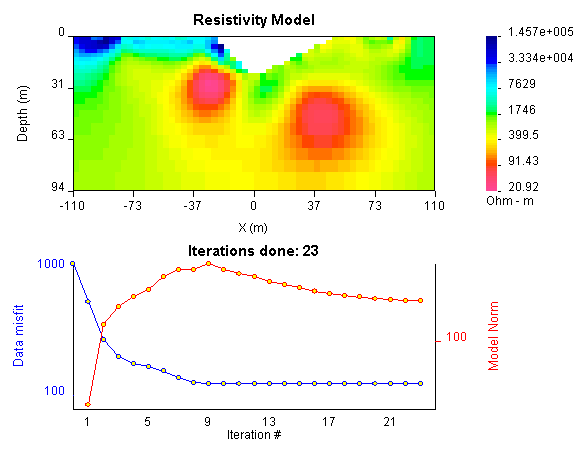
\includegraphics[width=0.5\columnwidth]{synHuber2}
\caption{(top) The recovered model from inversion of contaminated data using Huber norm for the data misfit and (b) the convergence curves.}
\label{fig:synInvHuber2}
\end{figure}

\subsection{IP Inversion of the forward model}
The inversion of IP data is almost identical to the inversion of DC resistivity data. The primary difference is that IP is a linear problem and the forward modeling matrix is the sensitivity matrix from the DC resistivity inversion. The IP inversion code has the same functionality as the DC resistivity code and the control lines are identical. One essential difference is that positivity is strictly enforced in the IP inversion. IP data can be negative but the intrinsic chargeability is always positive. There is no need to repeat all of the inversions done for the DC. Rather, we will invert only a few examples to illustrate the algorithm.
	
The inversion of IP data is almost identical to the inversion of DC resistivity data. The primary difference is that IP is a linear problem and the forward modeling matrix is the sensitivity matrix from the DC resistivity inversion. The IP inversion code has the same functionality as the DC resistivity code and the control lines are identical. One essential difference is that positivity is strictly enforced in the IP inversion. IP data can be negative but the intrinsic chargeability is always positive. There is no need to repeat all of the inversions done for the DC. Rather, we will invert only a few examples to illustrate the algorithm. 

The examples were designed to replicate the capabilities of \prog, shown using the DC examples. The conductivity models used for IP inversions were mainly those, acquired from the corresponding DC inversions.

\subsubsection{IP inversion: Zero-chargeability reference model}
The first example was carried out using zero-chargeability reference half space and the conductivity model acquired from inverting the dc resistivity with 1000 Ohm-m half space reference. The control file for this inversion is shown below:
%
\begin{fileExample}
\begin{tabular}{|ll|}
\hline
OBS LOC\_X obs\_ip.dat & ! IP data \\
TOPO FILE topo.dat & ! Topography\\
MESH FILE dcinv2d.msh & ! Mesh \\
ALPHA VALUE 1.e-3 1.0 1.0 & ! Alphas \\
INVMODE CG & ! Use CG \\
REF\_MOD FILE 1e-3 & ! Reference model \\
INIT\_MOD VALUE 1e-3 & ! Initial model \\
COND FILE dcinv2d.con & ! Recovered conductivity \\
\hline
\end{tabular}
\end{fileExample}
%
On the last line of this control file, there is the reference to the conductivity file, an essential input parameter for an IP inversion. This file has to come from a corresponding DC inversion, carried out prior to the IP inversion. The results of this inversion are shown in Figure \ref{fig:synIp1}.
%
\begin{figure}
\centering
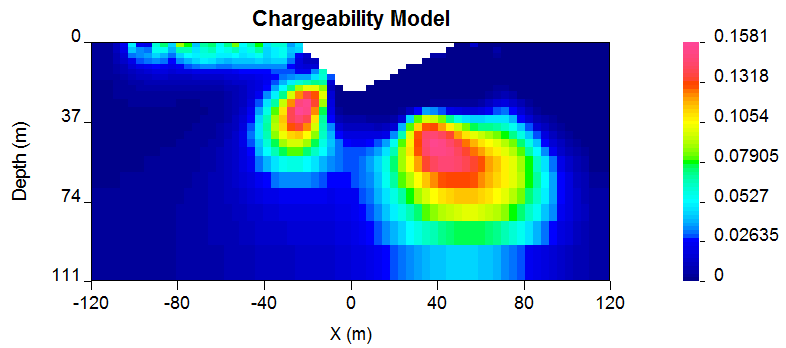
\includegraphics[width=0.5\columnwidth]{synIp1}
\caption{Recovered chargeability model for a zero chargeability reference model and 1000 Ohm-m conductivity model.}
\label{fig:synIp1}
\end{figure}

\subsubsection{IP inversion: Non-uniform reference model}
In the next example, similarly to the DC inversions, we have introduced a chargeable block into the reference model (Figure \ref{fig:synIPref}).
%
\begin{figure}
\centering
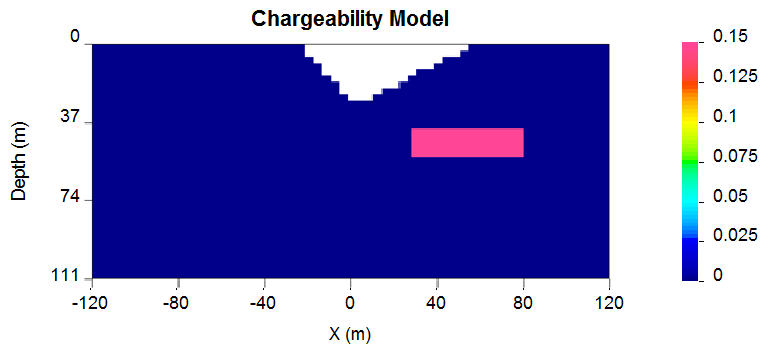
\includegraphics[width=0.5\columnwidth]{synIPref}
\caption{The reference model applied to the synthetic example for illustration.}
\label{fig:synIPref}
\end{figure}

Further, the new reference model was introduced in the inversion and omitted from the derivative terms. The control file for the inversion is virtually identical as in case with analogous inversion of the DC data and is provided below. The resulting inversion is shown in Figure \ref{fig:recSynIPref}.
%
\begin{fileExample}
\begin{tabular}{|ll|}
\hline
OBS LOC\_X obs\_ip.dat & ! IP data \\
TOPO FILE topo.dat & ! Topography\\
MESH FILE dcinv2d.msh & ! Mesh \\
ALPHA VALUE 1.e-2 1.0 1.0 & ! Alphas \\
INVMODE CG & ! Use CG \\
REF\_MOD FILE ref\_new.chg & ! Reference model \\
INIT\_MOD VALUE 1e-5 & ! Initial model \\
USE\_MREF FALSE & ! Ref mod only in smallness \\
COND FILE dcinv2d.con & ! Recovered conductivity \\
\hline
\end{tabular}
\end{fileExample}
%
\begin{figure}
\centering
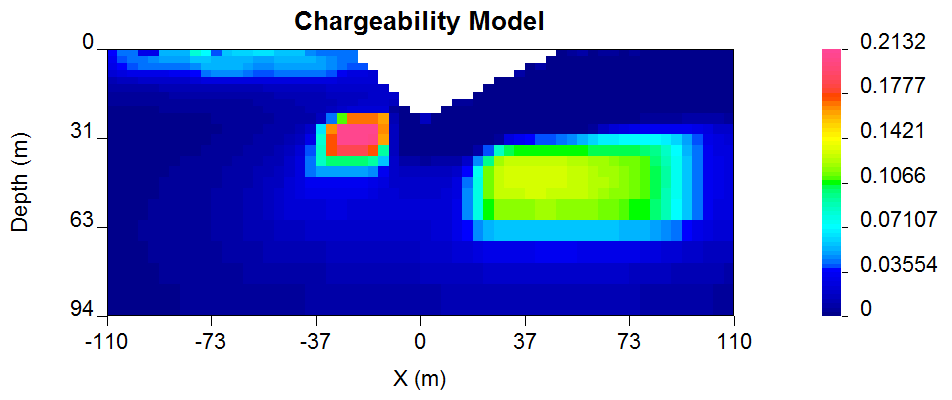
\includegraphics[width=0.5\columnwidth]{recSynIPref}
\caption{Recovered model from IP inversion using the non-uniform reference model in the smallness term.}
\label{fig:recSynIPref}
\end{figure}

\subsubsection{IP inversion: Using Ekblom measure to recover a blocky model}
In this next example, the geological information is incorporated in the model objective function using the $l_1$ norm measure rather than the default $l_2$ norm. This allows recovery of a blocky model. The control file for this example is provided below, and the resultant inversion model is shown in Figure \ref{fig:synIPblocky}.
%
\begin{fileExample}
\begin{tabular}{|ll|}
\hline
OBS LOC\_X obs\_ip.dat & ! IP data \\
TOPO FILE topo.dat & ! Topography\\
MESH FILE dcinv2d.msh & ! Mesh \\
ALPHA VALUE 1.e-3 1.0 1.0 & ! Alphas \\
INVMODE CG & ! Use CG \\
REF\_MOD FILE 1e-5 & ! Reference model \\
INIT\_MOD VALUE 1e-5 & ! Initial model \\
EKBLOM 1. 1. 1. 1.E-3 1.E-3 1.E-3 & ! Ekblom variables \\
COND FILE dcinv2d.con & ! Recovered conductivity \\
\hline
\end{tabular}
\end{fileExample}
%
\begin{figure}
\centering
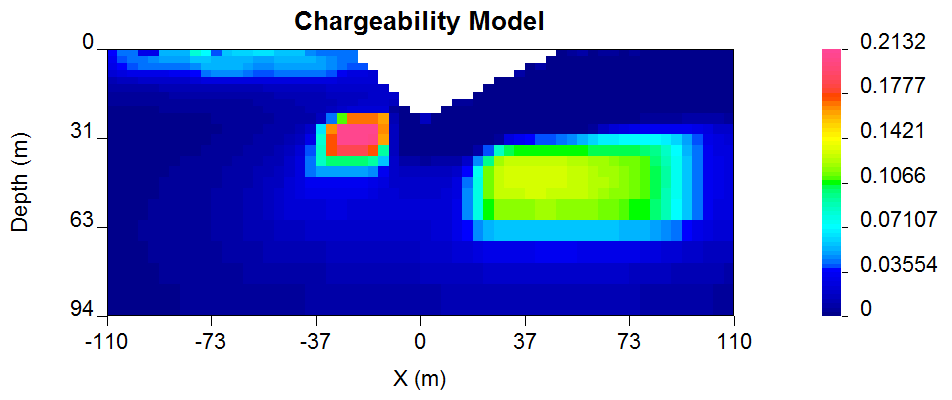
\includegraphics[width=0.5\columnwidth]{synIPblocky}
\caption{Recovered model from IP inversion Using $l_1$ measure (Ekblom norm) of model norm to recover a blocky model.}
\label{fig:synIPblocky}
\end{figure}

The resultant models are blocky and the central block has better defined boundaries than the deep block on the right. This arises because the right hand block is located close to the edge of the depth of investigation for the survey. To illustrate this we superpose the depth of investigation inferred by using the sensitivity function with a cutoff of 0.5. This is shown in Figure \ref{fig:synIPblockDOI} to illustrate the depth of investigation (DOI) the model has been plotted on a larger scale.
%
\begin{figure}
\centering
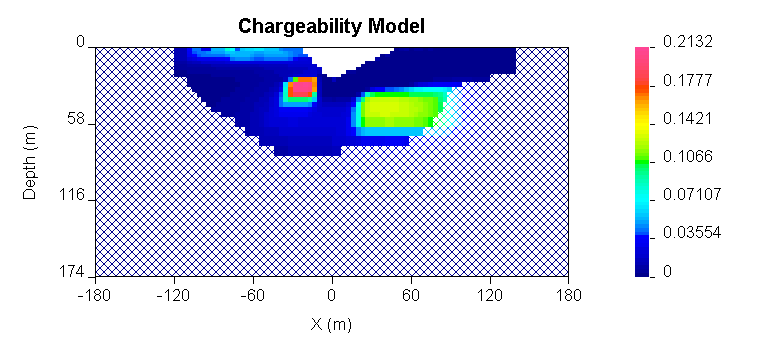
\includegraphics[width=0.5\columnwidth]{synIPblockDOI}
\caption{The depth of investigation (DOI) for the IP inversion with an $l_1$ model norm.}
\label{fig:synIPblockDOI}
\end{figure}

\subsubsection{IP inversion: Reference model with inactive cells}
This next example illustrates an inversion with a reference model with fixed cells (inactive). In this example, the inactive cells are representing a scenario when our constraints are acquired by incorporating borehole information. Out synthetic borehole is located on the profile at $x=60$ (Figure \ref{fig:synIPbore}a). This reference model is now different and involves only the knowledge we have from the borehole data (Figure \ref{fig:synIPbore}b). The inversion was carried out in the mode, when the inactive cells may influence their neighbours and resulted in the chargeability distribution shown in Figure \ref{fig:synIPbore}c. In this mode the inversion extends the chargeability of the fixed cells away from the reference block. The case is very similar to the analogous example shown in the DC inversion. The control file used for this inversion is provided below:
%
\begin{fileExample}
\begin{tabular}{|ll|}
\hline
OBS LOC\_X obs\_ip.dat & ! IP data \\
TOPO FILE topo.dat & ! Topography\\
MESH FILE dcinv2d.msh & ! Mesh \\
ALPHA LENGTH 100 100 & ! Length scales (m) \\
INVMODE CG & ! Use CG \\
REF\_MOD FILE new\_ref.chg & ! Reference model \\
ACTIVE\_CELLS active.txt & ! Active cell model \\
INIT\_MOD VALUE 1e-5 & ! Initial model \\
COND FILE dcinv2d.con & ! Recovered conductivity \\
\hline
\end{tabular}
\end{fileExample}
%

The \fileName{active} file is shown below, the structure has been edited so that two cells (one in each direction) around the synthetic borehole are set inactive and with the capability to influence the neighbours (i.e., -1)
\begin{fileExample}
\begin{tabular}{|cccccccccccccc|}
\hline
1 & 1 & 1 & 1 & 1 & 1 & -1 & -1 & 1 & 1 & 1 & 1 & 1 & 1 \\
1 & 1 & 1 & 1 & 1 & 1 & -1 & -1 & 1 & 1 & 1 & 1 & 1 & 1 \\
1 & 1 & 1 & 1 & 1 & 1 & -1 & -1 & 1 & 1 & 1 & 1 & 1 & 1 \\
1 & 1 & 1 & 1 & 1 & 1 & -1 & -1 & 1 & 1 & 1 & 1 & 1 & 1 \\
1 & 1 & 1 & 1 & 1 & 1 & -1 & -1 & 1 & 1 & 1 & 1 & 1 & 1 \\
1 & 1 & 1 & 1 & 1 & 1 & -1 & -1 & 1 & 1 & 1 & 1 & 1 & 1 \\
1 & 1 & 1 & 1 & 1 & 1 & -1 & -1 & 1 & 1 & 1 & 1 & 1 & 1 \\
\hline
\end{tabular}
\end{fileExample}
%
\begin{figure}
\centering
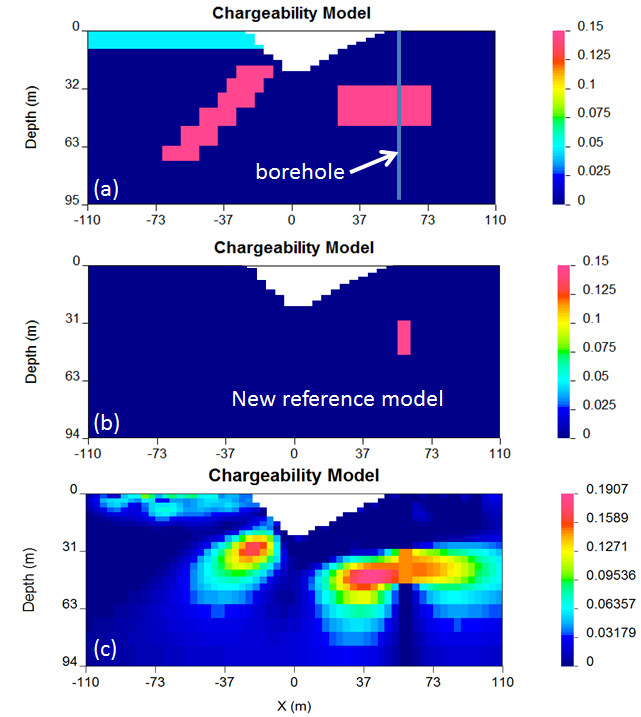
\includegraphics[width=0.5\columnwidth]{synIPbore}
\caption{(a) The true chargeability model with the borehole location. (b) The new reference model created from the borehole information. (c) Recovered model with the borehole locations set to inactive with influence (-1) on neighbouring cells.}
\label{fig:synIPbore}
\end{figure}

\subsection{Large data set example}
In the next example a synthetic data set is introduced, where a Wenner array is combined with a pole-dipole array and covers an 8-km long profile. The synthetic model is a 1000 Ohm- m half space covered by a 50-m thick overburden of variable electrical resistivity (200 Ohm-m section on the left, followed by 50 Ohm-m section in the middle, followed by 500 Ohm-m section on the right. The background resistive media is hosting two rectangular bodies at 150-m depth each. The prism on the left side is resistive (10,000 Ohm-m resistivity) and the prism on the right side is conductive (50 Ohm-m) (Figure \ref{fig:synLarge}a).

For the Wenner array the following configuration was used: number of stations = 400; minimum a-spacing = 80 m; maximum a-spacing 1367 m (spreading coefficient: 1.5 to accommodate up to 8 spreads per station). The spreading coefficient in this case is the multiplier used to calculate the increased spread distance between the potential electrodes for each station, given the minimum separation \fileName{a}) The total number of data for Wenner array (considering number of stations and all possible separations) was 2610 (Figure \ref{fig:synLarge}b).

The pole-dipole synthetic survey used a=75 m and n=1,10. The current pole was fixed on the right hand side of the array. This resulted in a total number of pole-dipole data of 1005 (Figure \ref{fig:synLarge}c). The combined Wenner and pole-dipole data set contains 3615 data (Figure \ref{fig:synLarge}d).

This synthetic model was discretized with a mesh, composed of 17918 cells (including padding), with the smallest cells reaching 30 m horizontally and 15 m vertically for the core region (depth to 1 km).
%
\begin{figure}
\centering
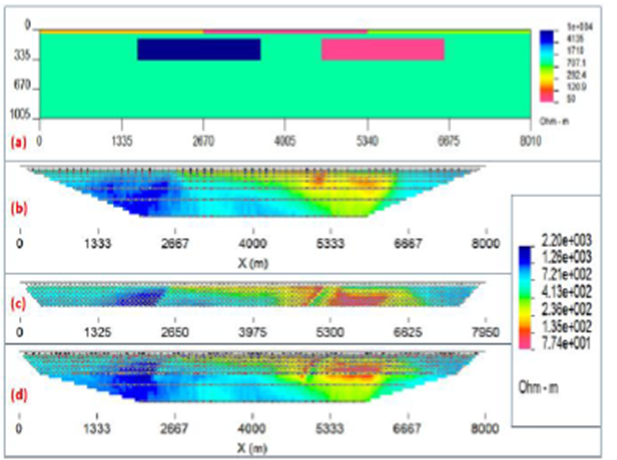
\includegraphics[width=0.5\columnwidth]{synLarge}
\caption{(a) The true model create for a large-scale synthetic data set by combining Wenner and Pole-dipole configurations. (b) The synthetic data from the Wenner array and (c) pole-dipole array are combined to get the (d) synthetic data for the entire data set.}
\label{fig:synLarge}
\end{figure}

This synthetic data set was contaminated with 5\% Gaussian noise and inverted using $l_1$ measure for model objective function in order to accommodate a more blocky inversion result. The inversion control file is provided below:
%
\begin{fileExample}
\begin{tabular}{|ll|}
\hline
OBS LOC\_X obs\_dc.dat & ! DC data \\
MESH FILE mesh2d.msh & ! Mesh \\
NITER 40 & ! Max iterations\\
INVMODE CG & ! Use CG \\
REF\_MOD FILE 1e-3 & ! Reference model \\
INIT\_MOD VALUE 1e-3 & ! Initial model \\
CHIFACT 1 & ! data misfit to number of data \\
EKBLOM 1. 1. 1. 1e-3 1e-3 1e-3 & ! Ekblom variables \\
BOUNDS 0.00001 0.02 & ! Global conductivity bounds \\
\hline
\end{tabular}
\end{fileExample}

The inversion converged in 17 iterations (Figure \ref{fig:synLargeRes}a) and was able to reconstruct all of the features shallower than 500-m of 	depth. This is consistent with the depth of investigation for this survey, based on the sensitivity (Figure \ref{fig:synLargeRes}b).
%
\begin{figure}
\centering
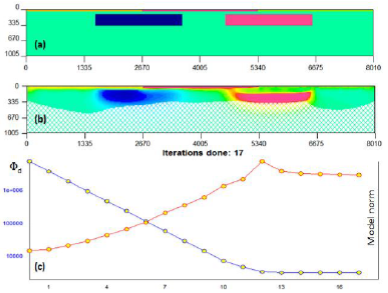
\includegraphics[width=0.5\columnwidth]{synLargeRec}
\caption{(a) The true model create for a large-scale synthetic data set by combining Wenner and Pole-dipole configurations. (b) The recovered model from inversion of the large synthetic data set with the Ekblom norm showing the DOI based on sensitivity analysis (threshold = 0.4). (c) The convergence curves show how the inversion performed.}
\label{fig:synLargeRes}
\end{figure}

The observed data were compared with the predicted data. The misfit is shown in Figure \ref{fig:synLargeMisfit}. The predicted data error does not exceed 3.9 standard deviations and overall data misfit is 3597.6.
%
\begin{figure}
\centering
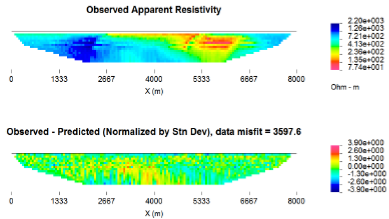
\includegraphics[width=0.5\columnwidth]{synLargeMisfit}
\caption{(a) Observed apparent resistivity (mixed Wenner/Pole-dipole data set) and the (b) data misfit, which is normalized by the standard deviation.}
\label{fig:synLargeMisfit}
\end{figure}

Finally, the parallelization of \prog~with OpenMP was analyzed on this example. It was inverted twice using 1 and 12 threads (6 cores with hyper-threading capability) with identical results. Running this example on one thread took 1:15:50.68 of CPU time, while running it on 6 cores (12 threads) resulted in convergence in 0:25:16.86 of CPU time, which is almost a threefold increase in productivity since the last release of \codeName{DCIP2D}.

%%%% BOREHOLE EXAMPLES %%%%
\input boreholeExample.tex
%%%%%%%%%%%%%%%%%%%%%%%%%%%

%%%%%% FIELD EXAMPLE %%%%%%
\input fieldExample.tex
%%%%%%%%%%%%%%%%%%%%%%%%%%%